%\section*{Appendix}
\label{sec:appendix}

\subsection*{Steps to start the Multimedia Frameworks and Codecs}

\subsubsection*{CVLC}
To start CVLC, follow the steps shown in Code Listing. \ref{cvlc}

\begin{lstlisting}[caption={Build and run CVLC}, frame=lines, label={cvlc}]
Navigate to the following directory:
/framework-test/ForRaspberryPi/cvlc

$docker build -t cvlc .

$docker run \
  -it \
  --privileged \
  --net=host -v /dev/video0:/dev/video0 \
  -e Ip=<IP of the Receiving Device> cvlc

h264:
$cvlc \
  -vvv v4l2:///dev/video0 \
  --sout "#transcode{vcodec=h264,
  width=640,
  fps=24,
  tune=zerolatency,
  preset=ultrafast}:udp{dst=<IP of the Receiving Device>:2000}" \
  --no-sout-audio

mjpeg:
$cvlc \
  -vvv v4l2:///dev/video0 \
  --sout "#transcode{vcodec=mjpg,
  fps=24}:udp{dst=<IP of the Receiving Device>:2000}" \
  --no-sout-audio

To view the video stream in VLC:
File->Open Network->Enter udp://@:2000
\end{lstlisting}

\subsubsection*{FFmpeg}
To start FFmpeg, follow the steps shown in Code Listing. \ref{ffmpeg}

\begin{lstlisting}[caption={Build and run Ffmpeg}, frame=lines, label={ffmpeg}]
Navigate to the following directory:
/framework-test/ForRaspberryPi/ffmpeg

$docker build -t ffmpeg .

$docker run \
  -it \
  --privileged \
  --net=host -v /dev/video0:/dev/video0 \
  -e Ip=<IP of the Receiving Device> ffmpeg
  
h264:
$ffmpeg \
  -fflags nobuffer \
  -f v4l2 \
  -framerate 30 \
  -i /dev/video0 \
  -vcodec libx264 \
  -preset ultrafast \
  -tune zerolatency \
  -pix_fmt yuv420p \
  -f mpegts udp://<IP of the Receiving Device>:2000?pkt_size=1316

mjpeg:
$ffmpeg \
  -fflags nobuffer \
  -f v4l2 \
  -framerate 30 \
  -i /dev/video0 \
  -vcodec mjpeg \
  -f mjpeg udp://<IP of the Receiving Device>:2000?pkt_size=1316

To view the video stream in VLC:
File->Open Network->Enter udp://@:2000
\end{lstlisting}

\subsubsection*{MJPG-Streamer}
To start MJPG-Streamer, follow the steps shown in Code Listing. \ref{mjpgstreamer}

\begin{lstlisting}[caption={Build and run MJPG-Streamer}, frame=lines, label={mjpgstreamer}]
Navigate to the following directory:
/framework-test/ForRaspberryPi/mjpgstreamer

docker build -t mjpgstreamer .

$docker run \
  -it \
  --privileged \
  --net=host \
  -v /dev/video0:/dev/video0 \
  -e Ip=<IP of the Receiving Device> mjpgstreamer

To view the video stream:
In browser: <IP of the Rpi>:8085
In vlc player: File->Open Network->Enter http://<IP of the Rpi>:8085/?action=stream
\end{lstlisting}

\subsubsection*{GStreamer}
To start GStreamer, follow the steps shown in Code Listing. \ref{gstreamer}

\begin{lstlisting}[caption={Build and run GStreamer}, frame=lines, label={gstreamer}]
To start Janus Server, navigate to the following directory:
/framework-test/ForReceivingDevice/janus_docker_for_testing

$docker run \
  --name=janus \
  --net=host \
  janus 
  
To start GStreamer, navigate to the following directory:
/framework-test/ForRaspberryPi/gstreamer

$docker build -t gstreamer .

$docker run \
  -it \
  --privileged \
  --net=host \
  -v /dev/video0:/dev/video0 \
  -e Ip=<IP of the Receiving Device> gstreamer

h264:
./gstreamer_h264.sh 

To view the video stream:
In browser: <Ip of the Rpi>
Demos->Streaming->Streams list->H.264 live stream(live)->Watch or Listen

To stop the video stream:
Stop
\end{lstlisting}

%Boxplots%
\subsection*{Boxplots showing the Utilization comparison of RPi3 and RPi4}
%CPU%
%\subsubsection{CPU}
\begin{figure}[H]
\centering
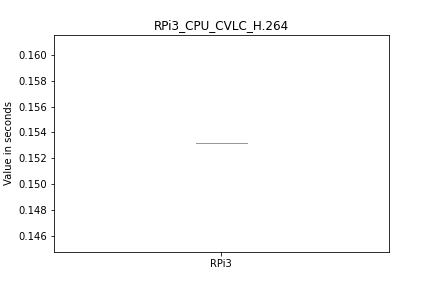
\includegraphics[width=.3\textwidth]{images/Boxplots/RPi3_CPU_CVLC_H_264.png}\hfill
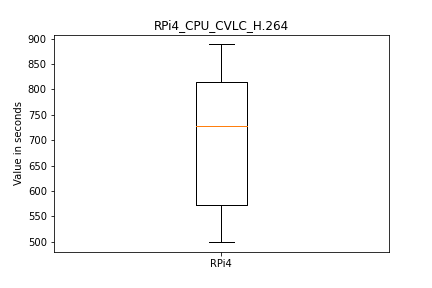
\includegraphics[width=.3\textwidth]{images/Boxplots/RPi4_CPU_CVLC_H_264.png}\hfill
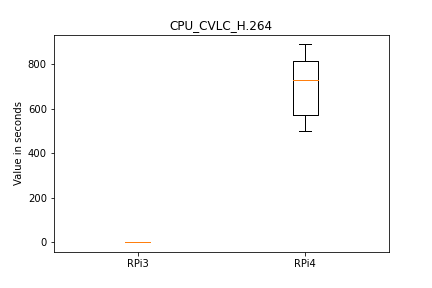
\includegraphics[width=.3\textwidth]{images/Boxplots/CPU_CVLC_H_264.png}
\caption{CPU CVLC H.264}
\label{fig:bp1}
\end{figure}

\begin{figure}[H]
\centering
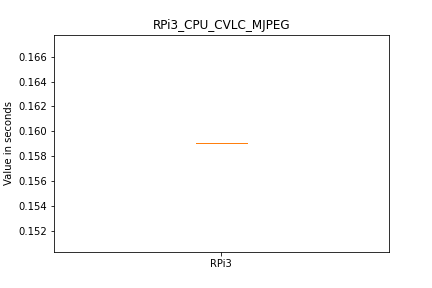
\includegraphics[width=.3\textwidth]{images/Boxplots/RPi3_CPU_CVLC_MJPEG.png}\hfill
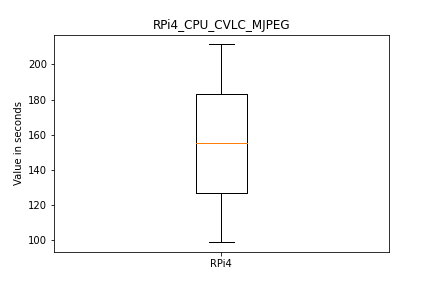
\includegraphics[width=.3\textwidth]{images/Boxplots/RPi4_CPU_CVLC_MJPEG.png}\hfill
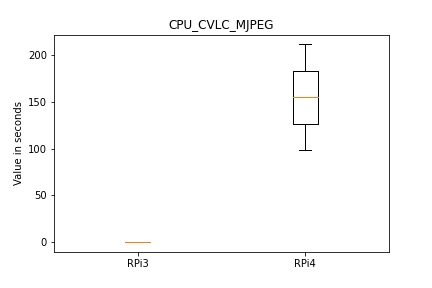
\includegraphics[width=.3\textwidth]{images/Boxplots/CPU_CVLC_MJPEG.png}
\caption{CPU CVLC MJPEG}
\label{fig:bp2}
\end{figure}

\begin{figure}[H]
\centering
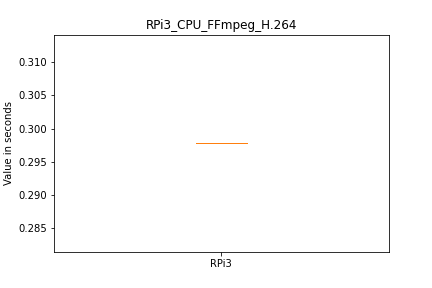
\includegraphics[width=.3\textwidth]{images/Boxplots/RPi3_CPU_FFmpeg_H_264.png}\hfill
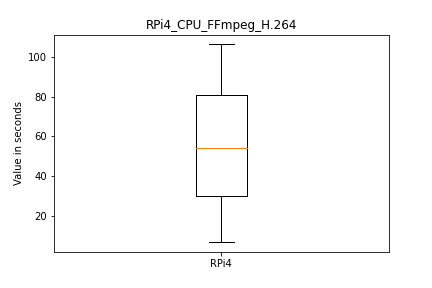
\includegraphics[width=.3\textwidth]{images/Boxplots/RPi4_CPU_FFmpeg_H_264.png}\hfill
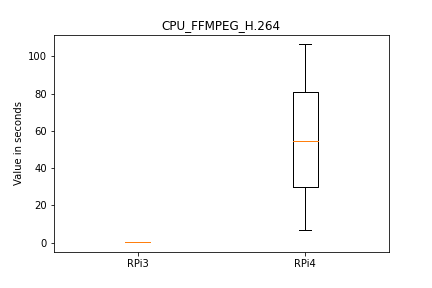
\includegraphics[width=.3\textwidth]{images/Boxplots/CPU_FFmpeg_H_264.png}
\caption{CPU FFmpeg H.264}
\label{fig:bp3}
\end{figure}
\clearpage

\begin{figure}[H]
\centering
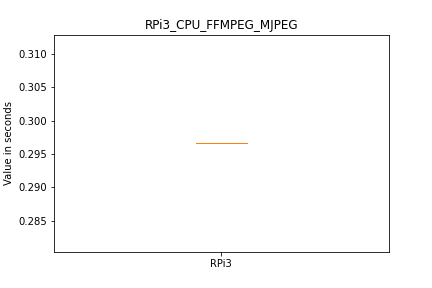
\includegraphics[width=.3\textwidth]{images/Boxplots/RPi3_CPU_FFmpeg_MJPEG.png}\hfill
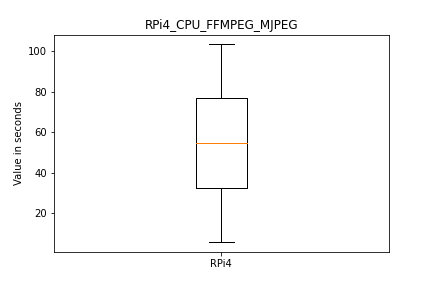
\includegraphics[width=.3\textwidth]{images/Boxplots/RPi4_CPU_FFmpeg_MJPEG.png}\hfill
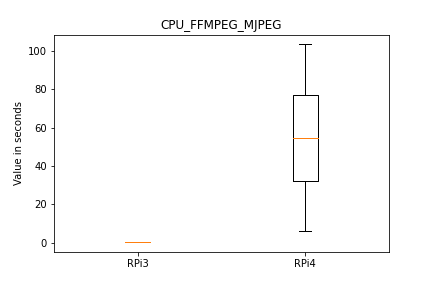
\includegraphics[width=.3\textwidth]{images/Boxplots/CPU_FFmpeg_MJPEG.png}
\caption{CPU FFmpeg MJPEG}
\label{fig:bp4}
\end{figure}

\begin{figure}[H]
\centering
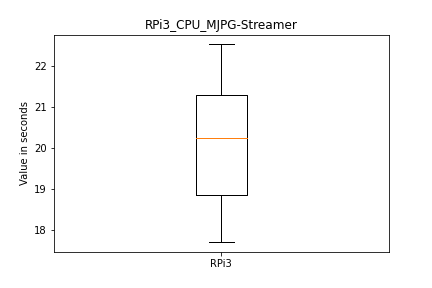
\includegraphics[width=.3\textwidth]{images/Boxplots/RPi3_CPU_MJPG-Streamer.png}\hfill
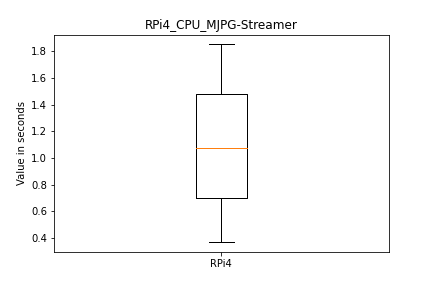
\includegraphics[width=.3\textwidth]{images/Boxplots/RPi4_CPU_MJPG-Streamer.png}\hfill
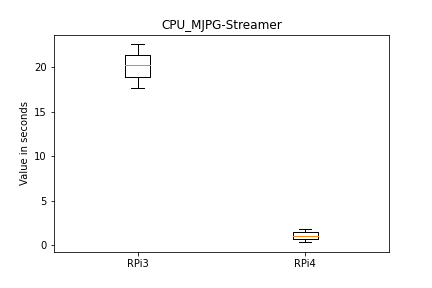
\includegraphics[width=.3\textwidth]{images/Boxplots/CPU_MJPG-Streamer.png}
\caption{CPU MJPG-Streamer}
\label{fig:bp5}
\end{figure}

\begin{figure}[H]
\centering
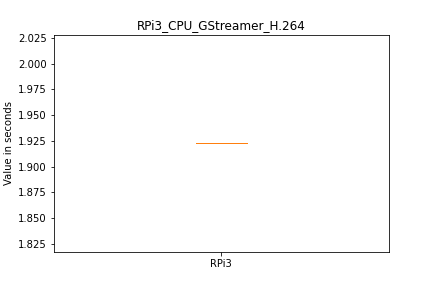
\includegraphics[width=.3\textwidth]{images/Boxplots/RPi3_CPU_GStreamer_H_264.png}\hfill
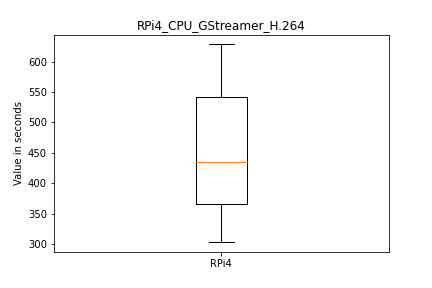
\includegraphics[width=.3\textwidth]{images/Boxplots/RPi4_CPU_GStreamer_H_264.png}\hfill
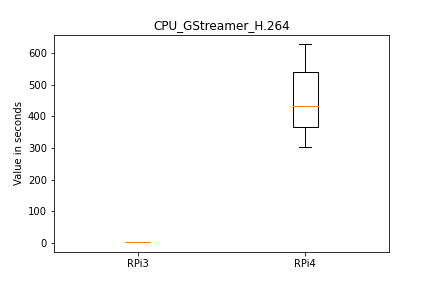
\includegraphics[width=.3\textwidth]{images/Boxplots/CPU_GStreamer_H_264.png}
\caption{CPU GStreamer H.264}
\label{fig:bp6}
\end{figure}

%Memory%
%\subsubsection{Memory}
\begin{figure}[H]
\centering
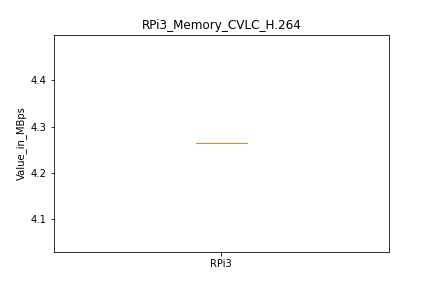
\includegraphics[width=.3\textwidth]{images/Boxplots/RPi3_Memory_CVLC_H_264.png}\hfill
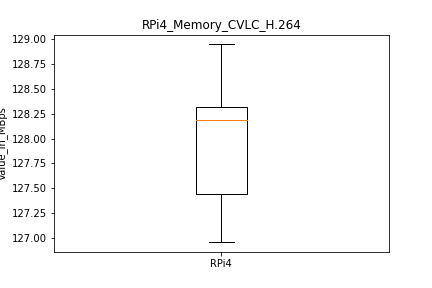
\includegraphics[width=.3\textwidth]{images/Boxplots/RPi4_Memory_CVLC_H_264.png}\hfill
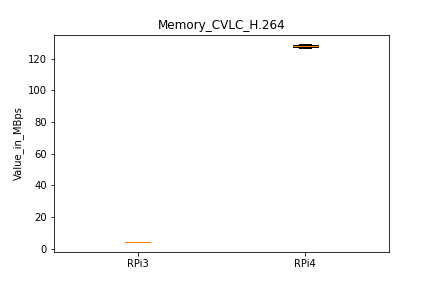
\includegraphics[width=.3\textwidth]{images/Boxplots/Memory_CVLC_H_264.png}
\caption{Memory CVLC H.264}
\label{fig:bp7}
\end{figure}

\begin{figure}[H]
\centering
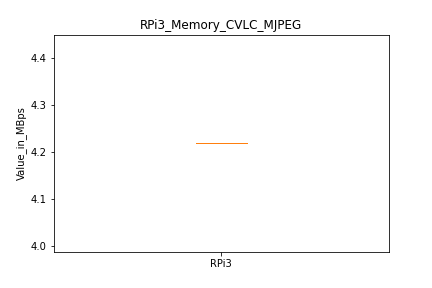
\includegraphics[width=.3\textwidth]{images/Boxplots/RPi3_Memory_CVLC_MJPEG.png}\hfill
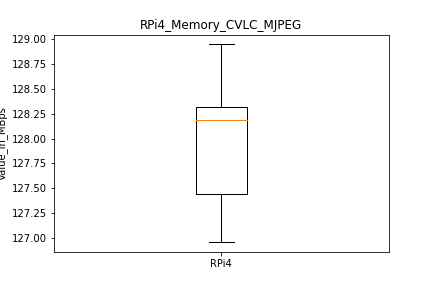
\includegraphics[width=.3\textwidth]{images/Boxplots/RPi4_Memory_CVLC_MJPEG.png}\hfill
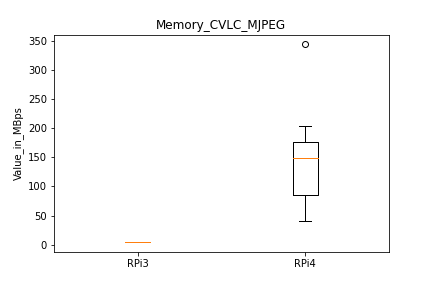
\includegraphics[width=.3\textwidth]{images/Boxplots/Memory_CVLC_MJPEG.png}
\caption{Memory CVLC MJPEG}
\label{fig:bp8}
\end{figure}
\clearpage

\begin{figure}[H]
\centering
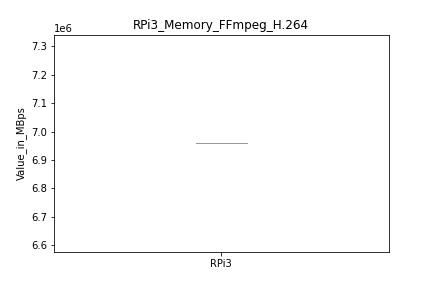
\includegraphics[width=.3\textwidth]{images/Boxplots/RPi3_Memory_FFmpeg_H_264.png}\hfill
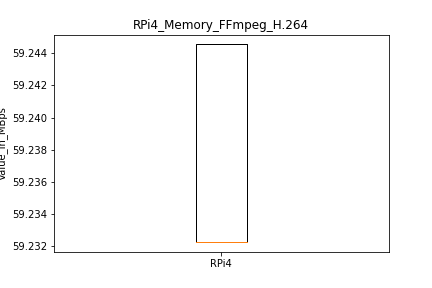
\includegraphics[width=.3\textwidth]{images/Boxplots/RPi4_Memory_FFmpeg_H_264.png}\hfill
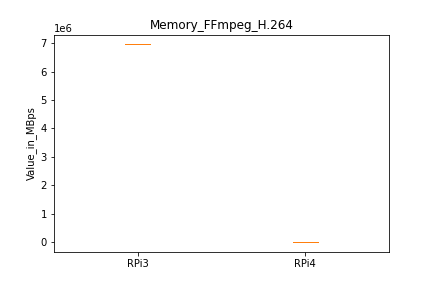
\includegraphics[width=.3\textwidth]{images/Boxplots/Memory_FFmpeg_H_264.png}
\caption{Memory FFmpeg H.264}
\label{fig:bp9}
\end{figure}

\begin{figure}[H]
\centering
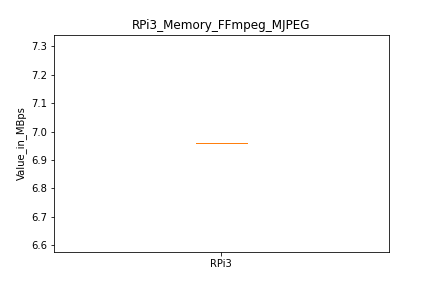
\includegraphics[width=.3\textwidth]{images/Boxplots/RPi3_Memory_FFmpeg_MJPEG.png}\hfill
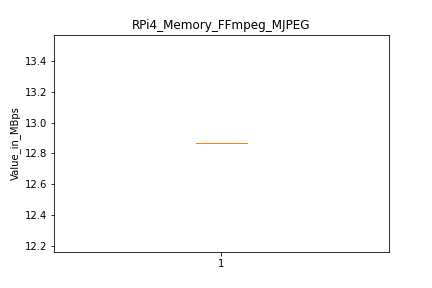
\includegraphics[width=.3\textwidth]{images/Boxplots/RPi4_Memory_FFmpeg_MJPEG.png}\hfill
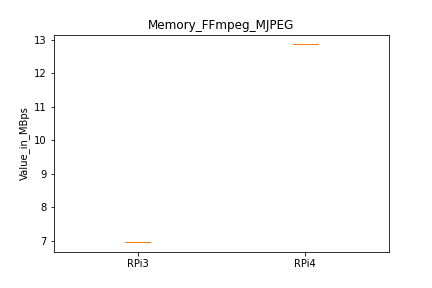
\includegraphics[width=.3\textwidth]{images/Boxplots/Memory_FFmpeg_MJPEG.png}
\caption{Memory FFmpeg MJPEG}
\label{fig:bp10}
\end{figure}

\begin{figure}[H]
\centering
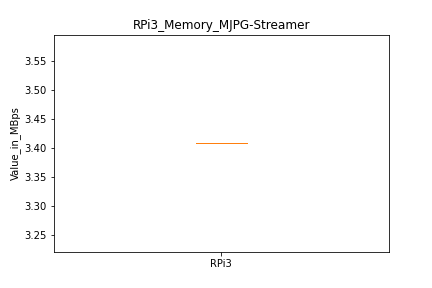
\includegraphics[width=.3\textwidth]{images/Boxplots/RPi3_Memory_MJPG-Streamer.png}\hfill
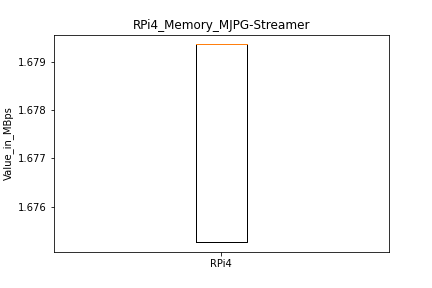
\includegraphics[width=.3\textwidth]{images/Boxplots/RPi4_Memory_MJPG-Streamer.png}\hfill
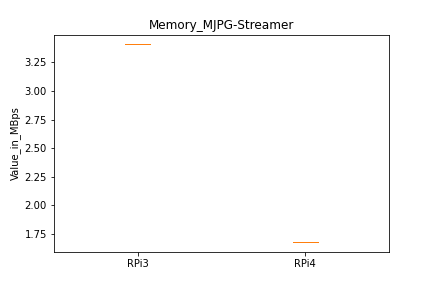
\includegraphics[width=.3\textwidth]{images/Boxplots/Memory_MJPG-Streamer.png}
\caption{Memory MJPG-Streamer}
\label{fig:bp11}
\end{figure}

\begin{figure}[H]
\centering
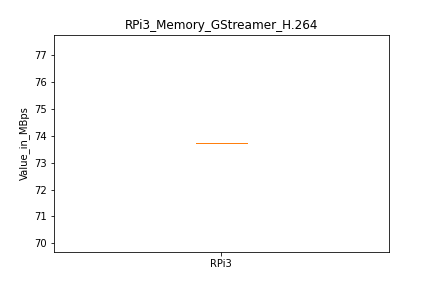
\includegraphics[width=.3\textwidth]{images/Boxplots/RPi3_Memory_GStreamer_H_264.png}\hfill
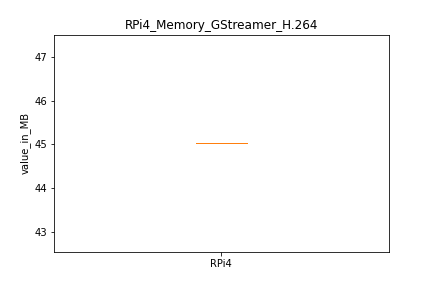
\includegraphics[width=.3\textwidth]{images/Boxplots/RPi4_Memory_GStreamer_H_264.png}\hfill
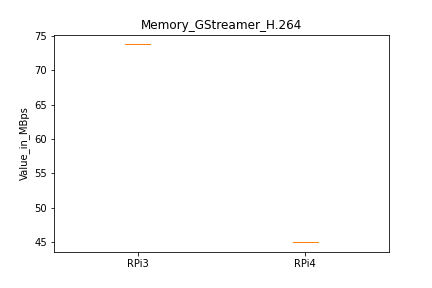
\includegraphics[width=.3\textwidth]{images/Boxplots/Memory_GStreamer_H_264.png}
\caption{Memory GStreamer H.264}
\label{fig:bp12}
\end{figure}

%Network Receive%
%\subsubsection{Network Receiver}
\begin{figure}[H]
\centering
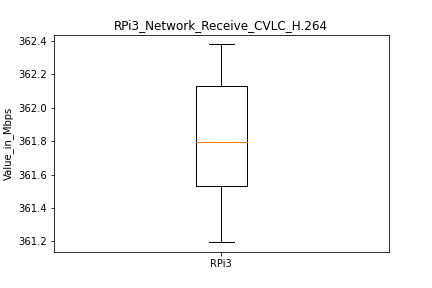
\includegraphics[width=.3\textwidth]{images/Boxplots/RPi3_Network_Receive_CVLC_H_264.png}\hfill
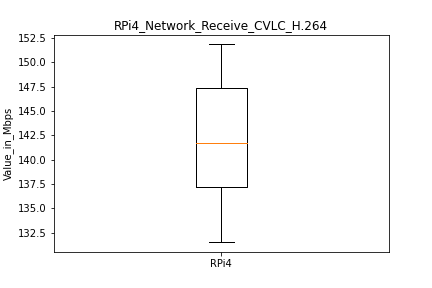
\includegraphics[width=.3\textwidth]{images/Boxplots/RPi4_Network_Receive_CVLC_H_264.png}\hfill
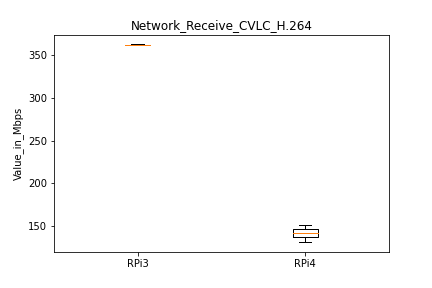
\includegraphics[width=.3\textwidth]{images/Boxplots/Network_Receive_CVLC_H_264.png}
\caption{Network Receive CVLC H.264}
\label{fig:bp13}
\end{figure}
\clearpage

\begin{figure}[H]
\centering
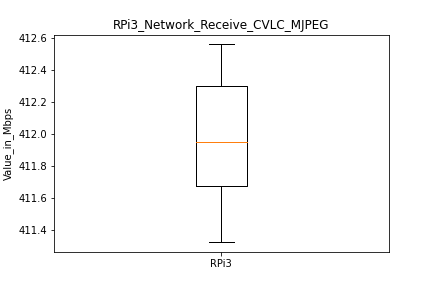
\includegraphics[width=.3\textwidth]{images/Boxplots/RPi3_Network_Receive_CVLC_MJPEG.png}\hfill
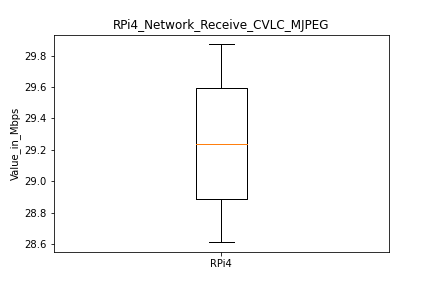
\includegraphics[width=.3\textwidth]{images/Boxplots/RPi4_Network_Receive_CVLC_MJPEG.png}\hfill
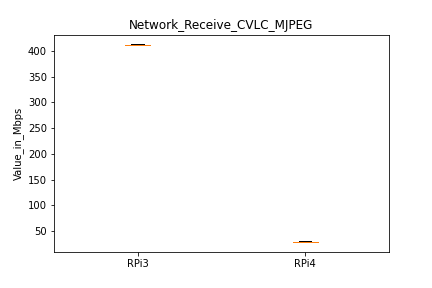
\includegraphics[width=.3\textwidth]{images/Boxplots/Network_Receive_CVLC_MJPEG.png}
\caption{Network Receive CVLC MJPEG}
\label{fig:bp14}
\end{figure}

\begin{figure}[H]
\centering
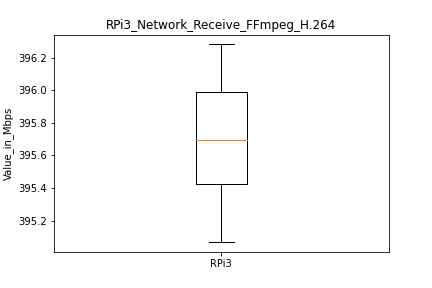
\includegraphics[width=.3\textwidth]{images/Boxplots/RPi3_Network_Receive_FFmpeg_H_264.png}\hfill
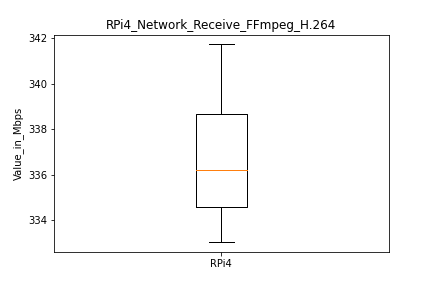
\includegraphics[width=.3\textwidth]{images/Boxplots/RPi4_Network_Receive_FFmpeg_H_264.png}\hfill
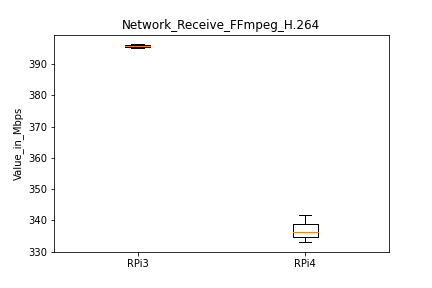
\includegraphics[width=.3\textwidth]{images/Boxplots/Network_Receive_FFmpeg_H_264.png}
\caption{Network Receive FFmpeg H.264}
\label{fig:bp14}
\end{figure}

\begin{figure}[H]
\centering
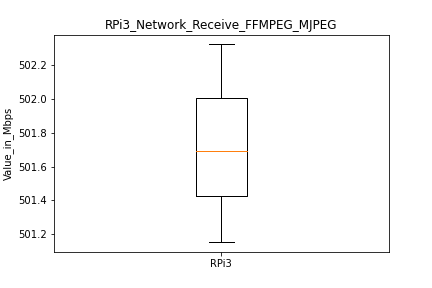
\includegraphics[width=.3\textwidth]{images/Boxplots/RPi3_Network_Receive_FFmpeg_MJPEG.png}\hfill
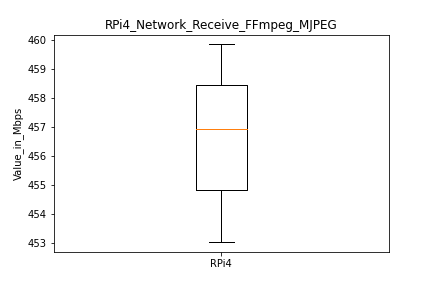
\includegraphics[width=.3\textwidth]{images/Boxplots/RPi4_Network_Receive_FFmpeg_MJPEG.png}\hfill
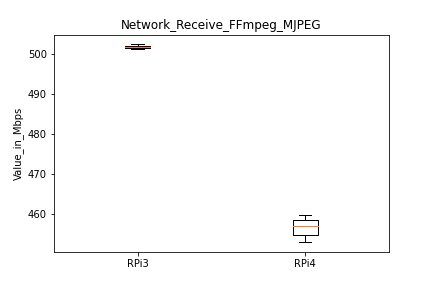
\includegraphics[width=.3\textwidth]{images/Boxplots/Network_Receive_FFmpeg_MJPEG.png}
\caption{Network Receive FFmpeg MJPEG}
\label{fig:bp15}
\end{figure}

\begin{figure}[H]
\centering
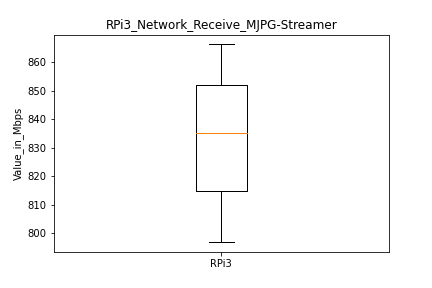
\includegraphics[width=.3\textwidth]{images/Boxplots/RPi3_Network_Receive_MJPG-Streamer.png}\hfill
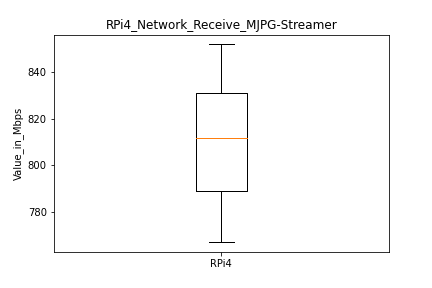
\includegraphics[width=.3\textwidth]{images/Boxplots/RPi4_Network_Receive_MJPG-Streamer.png}\hfill
\includegraphics[width=.3\textwidth]{images/Boxplots/Network_Receive_MJPG-Streamer.png}
\caption{Network Receive MJPG-Streamer}
\label{fig:bp16}
\end{figure}

\begin{figure}[H]
\centering
\includegraphics[width=.3\textwidth]{images/Boxplots/RPi3_Network_Receive_GStreamer.png}\hfill
\includegraphics[width=.3\textwidth]{images/Boxplots/RPi4_Network_Receive_GStreamer.png}\hfill
\includegraphics[width=.3\textwidth]{images/Boxplots/Network_Receive_GStreamer_H_264.png}
\caption{Network Receive GStreamer H.264}
\label{fig:bp17}
\end{figure}

%Network Tranmsit%
%\subsubsection{Network Tranmsit}
\begin{figure}[H]
\centering
\includegraphics[width=.3\textwidth]{images/Boxplots/RPi3_Network_Transmit_CVLC_H_264.png}\hfill
\includegraphics[width=.3\textwidth]{images/Boxplots/RPi4_Network_Transmit_CVLC_H_264.png}\hfill
\includegraphics[width=.3\textwidth]{images/Boxplots/Network_Transmit_CVLC_H_264.png}
\caption{Network Transmit CVLC H.264}
\label{fig:bp18}
\end{figure}

\begin{figure}[H]
\centering
\includegraphics[width=.3\textwidth]{images/Boxplots/RPi3_Network_Transmit_CVLC_MJPEG.png}\hfill
\includegraphics[width=.3\textwidth]{images/Boxplots/RPi4_Network_Transmit_CVLC_MJPEG.png}\hfill
\includegraphics[width=.3\textwidth]{images/Boxplots/Network_Transmit_CVLC_MJPEG.png}
\caption{Network Transmit CVLC MJPEG}
\label{fig:bp19}
\end{figure}

\begin{figure}[H]
\centering
\includegraphics[width=.3\textwidth]{images/Boxplots/RPi3_Network_Transmit_FFmpeg_H_264.png}\hfill
\includegraphics[width=.3\textwidth]{images/Boxplots/RPi4_Network_Transmit_FFmpeg_H_264.png}\hfill
\includegraphics[width=.3\textwidth]{images/Boxplots/Network_Transmit_FFmpeg_H_264.png}
\caption{Network Transmit FFmpeg H.264}
\label{fig:bp20}
\end{figure}

\begin{figure}[H]
\centering
\includegraphics[width=.3\textwidth]{images/Boxplots/RPi3_Network_Transmit_FFmpeg_MJPEG.png}\hfill
\includegraphics[width=.3\textwidth]{images/Boxplots/RPi4_Network_Transmit_FFmpeg_MJPEG.png}\hfill
\includegraphics[width=.3\textwidth]{images/Boxplots/Network_Transmit_FFmpeg_MJPEG.png}
\caption{Network Transmit FFmpeg MJPEG}
\label{fig:bp21}
\end{figure}

\begin{figure}[H]
\centering
\includegraphics[width=.3\textwidth]{images/Boxplots/RPi3_Network_Transmit_MJPG-Streamer.png}\hfill
\includegraphics[width=.3\textwidth]{images/Boxplots/RPi4_Network_Transmit_MJPG-Streamer.png}\hfill
\includegraphics[width=.3\textwidth]{images/Boxplots/Network_Transmit_MJPG-Streamer.png}
\caption{Network Transmit MJPG-Streamer}
\label{fig:bp22}
\end{figure}

\begin{figure}[H]
\centering
\includegraphics[width=.3\textwidth]{images/Boxplots/RPi3_Network_Transmit_GStreamer_H_264.png}\hfill
\includegraphics[width=.3\textwidth]{images/Boxplots/RPi4_Network_Transmit_GStreamer_H_264.png}\hfill
\includegraphics[width=.3\textwidth]{images/Boxplots/Network_Transmit_GStreamer_H_264.png}
\caption{Network Transmit GStreamer H.264}
\label{fig:bp23}
\end{figure}